% Chapter 4

\chapter{Experimental Results} % Main chapter title

\label{Chapter4} % For referencing the chapter elsewhere, use \ref{Chapter4} 


%----------------------------------------------------------------------------------------
\section{Historical validation of topics}
% word distributions of a topic over time

% area chart of cumulative topic percentages in class over time. (i.e. add up all the vectors, normalize ot total amount, find percent, repeat for each epoch.)

%----------------------------------------------------------------------------------------
%\section{DIM Results and Insights}
%\subsection{Influence Metric}
%\subsubsection{validating influential patents}
%\subsubsection{correlation with forward citations}
%\subsubsection{correlation with page-rank}

%----------------------------------------------------------------------------------------
\section{Coherence Testing}

\begin{table}[ht]
\caption[Coherences]{The coherence values of each model}
\label{tab:coherences}
\centering
\begin{tabular}{l l l l l}
\toprule
\tabhead{Model} & \tabhead{c$\_$v} & \tabhead{c$\_$uci} & \tabhead{c$\_$npmi} & \tabhead{u$\_$mass} \\
\midrule
LDA & .5021 & .1904 & .0750 & -1.6283 \\
DTM & .5980 & .4373 & .1213 & -1.6688 \\
DIM & .5581 & .2865 & .1011 & -1.3478 \\
\bottomrule\\
\end{tabular}
\end{table}


\begin{figure}[h]
\centering
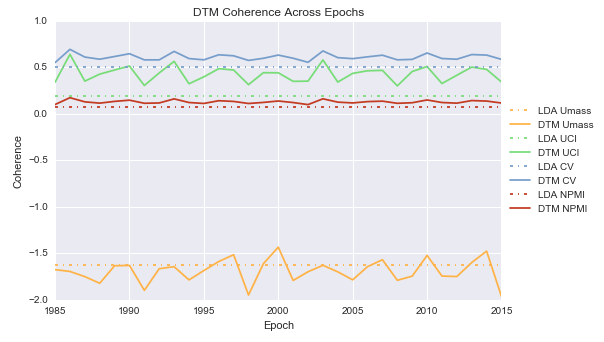
\includegraphics[width=130mm,scale=0.45]{Figures/DTMCoherences}
\decoRule
\caption[EpochCoherences]{Coherence scores for the DTM and LDA across epochs}
\label{fig:EpochCoherences}
\end{figure}


%----------------------------------------------------------------------------------------
\section{Classification Results}

% they cite the normalized mutual information equation! use those!
The clustering result is evaluated by comparing the Normalized mutual information (Xu et al. 2003; Cai et al. 2008) [NEED TO ACTUALLY CITE]
%Xu, W., Liu, X., & Gong, Y. (2003). Document clustering based on non-negative matrix factorization. In
%SIGIR ’03: Proceedings of the 26th annual international ACM SIGIR conference on research and
%development in informaion retrieval (pp. 267–273). New York, NY, USA: ACM.
%Cai, D., Mei, Q., Han, J., & Zhai, C. (2008). Modeling hidden topics on document manifold. In
%J. G. Shanahan, S. Amer-Yahia, I. Manolescu, Y. Zhang, D. A. Evans, A. Kolcz, K.-S. Choi, &
%A. Chowdhury (Eds.), CIKM (pp. 911–920). ACM.

\section{Clustering Results}

